\documentclass[12pt]{article}

% 中文支持
\usepackage{ctex}

% 页边距设置
\usepackage[a4paper, margin=1in]{geometry}

% 数学公式支持
\usepackage{amsmath, amssymb}

% 图片支持
\usepackage{graphicx}

% 表格支持
\usepackage{array}

% 超链接支持
\usepackage[linkcolor=blue, anchorcolor=blue, citecolor=blue]{hyperref}

\usepackage{caption}
\usepackage{subcaption}
\usepackage{booktabs}
\usepackage{tabularx}
\usepackage{float}

\newcommand{\keywords}[1]{\textbf{关键词:} #1}
% 自定义标题
\title{\fontsize{16pt}{16pt}\selectfont 基于ARMA-GARCH与VAR模型的中信证券股票收益率分析}
\author{田晨楷 2211333}
\date{\today}

\begin{document}

% 生成标题
\maketitle

\begin{abstract}
本文聚焦于中信证券股票、行业金融指数及上证指数,通过对其长达六年的日交易数据进行详尽剖析,我们试图揭示中信证券股票收益率波动性的ARCH现象。为深入挖掘这一波动特性的内在机理,我们构建了ARMA-GARCH模型作为研究框架,并搭建了连接中信证券收益率与金融行业指数、上证指数的动态VAR模型体系。研究发现,中信证券的收益率波动对金融行业整体表现及上证指数波动有显著影响,VAR模型展现了对这些外部冲击因素的高效捕捉与解析能力。随后,我们进行了脉冲响应分析,巩固了模型在阐释市场动态冲击及波动传导路径上的有效性。最后,我们进行了Granger因果检验,捕捉了中信证券股票收益率与行业金融指数和上证指数之间的即时因果关系

综上所述,本文不仅深化了对中信证券股票收益率波动性及其市场驱动因素的认识,更为市场参与者与投资决策者提供了基于实证分析的精准市场预测与风险管理策略参考。

\keywords{股票收益率\quad 时间序列分析\quad ARMA-GARCH模型\quad VAR模型\quad 白噪声检验\quad 脉冲响应分析\quad Granger因果检验}

\end{abstract}

\newpage
\tableofcontents

\newpage
\section{引言}
股票市场是金融市场的重要组成部分,对推动国民经济发展和世界一体化影响重大。对于股票收益率的预测是金融研究的一个重大研究方向。近年来,股票市场规模快速扩大,市场透明度也越来越高,投资者的交易策略同质化严重,股票价格的预测变得更加困难,因此,为了更好地预测股票价格的走势,探讨合理有效的预测方法十分重要。为了更好地理解和解释股票收益率的波动性,并提供有效的风险管理和投资决策支持,学者们广泛应用各种时间序列模型,最为典型的当属自回归移动平均模型(AutoRegressive Moving Average, ARMA)、广义自回归条件异方差模型(Generalized Autoregressive Conditional Heteroskedasticity, GARCH)及向量自回归模型(Vector AutoRegressive model, VAR)。

中信证券是国内首家、也是唯一一家资产规模突破万亿的证券公司,是金融行业的领头羊。作为证券行业的龙头企业,中信证券的股价能够反映其行业地位和整体竞争力,能体现投资者的信心和整体市场情绪,具有代表性。因此,我们决定选取中信证券股票的收盘价和收益率作为主要研究对象。

\subsection{问题来源}
我们选择问题的契机源自一篇实证论文《基于ARMA-GARCH模型的上证综指收益率研究》。这篇论文选取了2015至2020年上证综指的日收盘价,基于ARMA-GARCH模型研究了上证综指收益率。结果表明,上证综指对数收益率序列存在波动聚集性,且模型对短期预测效果优于长期。这篇论文启发我们利用ARMA-GARCH模型等时间序列模型,更加深刻地理解股票市场的波动特征。基于计量模型的角度研究股票市场的影响因素一直是股票市场的重要研究方向之一,这也符合我们把实证分析与金融问题相结合的研究意图。

\subsection{选题理由}
我们希望能为股票市场的投资者和决策者提供市场预测和风险管理支持,为更好地理解和解释股票收益率的波动性做出边际贡献。因此,经过深入讨论,考虑到样本的数量和典型性,我们决定在原论文的基础上更进一步——不仅分析某只股票收益率的波动性,也考虑股票收益率与行业及上证指数波动关联的显著性。VAR模型能有效捕捉这些影响,脉冲响应能分析验证模型对市场冲击和波动传导的解释能力。最终,我们决定选择中信证券股票、行业金融指数和上证指数的收盘价和收益率,利用ARMA-GARCH和VAR模型研究股票收益率的波动性。


\section{问题分析}

\subsection{样本数据}

本研究涵盖了2018年1月2日至2024年6月28日的样本数据,涉及中信证券、行业金融指数和上证指数的收盘价和收益率数据。

\subsection{变量定义}

在本次实证研究中,我们选取了三个主要变量:中信证券(ZX)、行业金融指数(JRIdx)和上证指数(SZIdx)。这些变量的定义包括收盘价和收益率两个关键指标。收盘价是每日交易结束时股票或指数的价格,而收益率则用于衡量股票或指数在相邻两个交易日之间的价格变化情况。

收盘价数据直接从各个交易日的市场数据中获取,用于描述股票或指数的绝对价格水平。对于收益率的计算,我们采用对数收益率的定义,即$ln$(本期收盘价/上期收盘价)。这种对数收益率的计算方法在金融时间序列分析中有广泛应用,因为它具有多种统计优势,包括正态性更强、时间可加性以及更适合处理大幅波动的数据。

\subsection{逻辑框架}
我们的主要目标是:

\begin{itemize}
    \item 验证中信证券股票收益率的波动率是否存在ARCH效应
    \item 探索ARMA-GARCH模型对中信证券股票收益率波动性的解释能力
    \item 验证中信证券收益率是否与行业指数及上证指数显著相关
    \item 探索VAR模型能否有效捕捉市场间的动态相互作用
    \item 更深刻地理解和解释股票收益率的波动特征
\end{itemize}

我们通过以下4个部分实现这些目标:

\begin{itemize}
    \item \textbf{Part 1:描述性统计}
\end{itemize}

对股票观测数、均值、标准差、最小值、中位数、最大值进行统计。


\begin{itemize}
    \item \textbf{Part 2:ARMA模型分析}
\end{itemize}

在这个部分,我们依次进行了如下分析操作。

\begin{itemize}
    \item[$\ast$] 平稳性检验
\end{itemize}

\begin{itemize}
    \item[$\ast$] 白噪声检验
\end{itemize}

\begin{itemize}
    \item[$\ast$] 使用AIC、BIC等信息准则进行模型定阶
\end{itemize}

\begin{itemize}
    \item[$\ast$] 构建AR(3)、MA(3)、ARMA(3,3)模型,捕捉股票收益率的自相关和滑动平均关系
\end{itemize}

\begin{itemize}
    \item[$\ast$] 验证拟合残差序列是否为白噪声序列
\end{itemize}

\begin{itemize}
    \item \textbf{Part 3:GARCH模型分析}
\end{itemize}


在这个部分,我们依次进行了如下分析操作。

\begin{itemize}
    \item[$\ast$] 自相关性分析
\end{itemize}

\begin{itemize}
    \item[$\ast$] 探索股票收益率的波动性聚集特征
\end{itemize}

\begin{itemize}
    \item[$\ast$] 验证股票收益率的波动率是否存在ARCH效应
\end{itemize}

\begin{itemize}
    \item[$\ast$] 使用AIC、BIC等信息准则进行模型定阶
\end{itemize}

\begin{itemize}
    \item[$\ast$] 构建GARCH(4,0)模型
\end{itemize}

\begin{itemize}
    \item[$\ast$] 稳健性检验
\end{itemize}

\begin{itemize}
    \item \textbf{Part 4:VAR模型分析}
\end{itemize}

在这个部分,我们依次进行了如下分析操作。

\begin{itemize}
    \item[$\ast$] 平稳性检验
\end{itemize}

\begin{itemize}
    \item[$\ast$] 使用AIC、BIC等信息准则进行模型定阶
\end{itemize}

\begin{itemize}
    \item[$\ast$] 构建VAR模型的回归方程
\end{itemize}

\begin{itemize}
    \item[$\ast$] 自相关性分析
\end{itemize}

\begin{itemize}
    \item[$\ast$] 脉冲响应分析
\end{itemize}

\begin{itemize}
    \item[$\ast$] Granger因果检验
\end{itemize}

\section{结果展示}

\subsection{描述性统计}
我们对中信证券、行业金融指数和上证指数的收盘价和收益率进行描述性统计,以探讨这些指标的特性及其差异。中信证券的收盘价平均值为22.17元,标准差为3.71,最小值为14.84元,最大值为33.5元。四分位数分别为19.57元、21.66元和24.15元。相比之下,行业金融指数和上证指数的收盘价均值和波动性明显更高。行业金融指数的平均收盘价为1170.46,标准差为189.64,四分位数分别为1043.18、1145.92和1324.09,最小值和最大值分别为740.16和1589.01。上证指数的平均收盘价为3147.90,标准差为267.98,四分位数分别为2954.38、3142.78和3340.29,最小值和最大值分别为2486.42和3715.37。相对于中信证券,行业金融指数和上证指数在研究期间表现出了更大的波动性和更高的价格水平。

中信证券的平均收益率接近于零(1.20E-05),标准差为0.0201,最小值和最大值分别为-0.1055和0.0954。四分位数分别为-0.0101、-0.0006和0.0093。行业金融指数的平均收益率为-0.0001083,标准差为0.0169,四分位数分别为-0.0092、-0.0009和0.0077,最小值和最大值分别为-0.0995和0.0899。上证指数的平均收益率为-3.09E-05,标准差为0.0108,四分位数分别为-0.0055、0.0001和0.0058,最小值和最大值分别为-0.0804和0.0555。相较于中信证券,行业金融指数和上证指数的收益率波动性较小,尤其是上证指数,其收益率的标准差最小。中信证券的股票收益率在研究期间具有较高的波动性,而上证指数的整体市场波动相对较小。

结果如表\ref{tab:summary stats}所示。

\begin{table}[H]
    \centering
    \caption{描述性统计}
    \label{tab:summary stats}
    \begin{tabular}{ccccccc}
        \toprule
变量名 & 观测数 & 均值 & 标准差 & 最小值 & 中位数 & 最大值\\
        \midrule
中信证券收益率 & 1545 & 0.0000    & 0.0201   & -0.1055   & -0.0006   & 0.0954    \\
中信证券收盘价 & 1545 & 22.1690   & 3.7065   & 14.8400   & 21.6600   & 33.5000   \\
上证指数收益率 & 1545 & 0.0000    & 0.0108   & -0.0804   & 0.0001    & 0.0555    \\
上证指数收盘价 & 1545 & 3147.8986 & 267.9755 & 2486.4186 & 3142.7790 & 3715.3723 \\
金融指数收益率 & 1545 & -0.0001   & 0.0169   & -0.0995   & -0.0009   & 0.0899    \\
金融指数收盘价 & 1545 & 1170.4551 & 189.6384 & 740.1551  & 1145.9184 & 1589.0097 \\
        \bottomrule
    \end{tabular}
\end{table}

\subsection{ARMA模型}
首先,我们采用Phillips-Perron单位根检验验证中信证券收益率的平稳性,所得$p$值为0.01,故拒绝原假设,接受备择假设,即所采用的中信证券对数收益率序列为平稳序列。

之后,我们对其进行白噪声检验——Portmanteau(Q) test与Bartlett's(B) test。值得注意的是,我们求得Portmanteau(Q) test与Bartlett's(B) test 的$p$值均接近于1,故无法拒绝原假设,即应认为序列为白噪声序列,这一检验结果与所参考论文严重不符。对于纯随机序列,又称白噪声序列,序列的各项数值之间没有任何相关关系,序列在进行完全无序的随机波动,是没有信息可提取的平稳序列,因此无法运用ARMA模型。但是,基于对文献进行进一步验证的目的,我们仍继续按论文中的方法,采用ARMA模型捕捉中信证券收益率的自相关和滑动平均关系。

在正式分析之前要选择合适的ARMA模型阶数,我们采用相关系数初步判断参数,后续通过稳健性检验与AIC、BIC等信息准则综合选取参数进行模型定阶。

我们绘制了中信证券和收益率的时序图\ref{fig:A1}、自相关图和偏自相关图\ref{fig:A23},如图所示:

\begin{figure}[H]
\centering
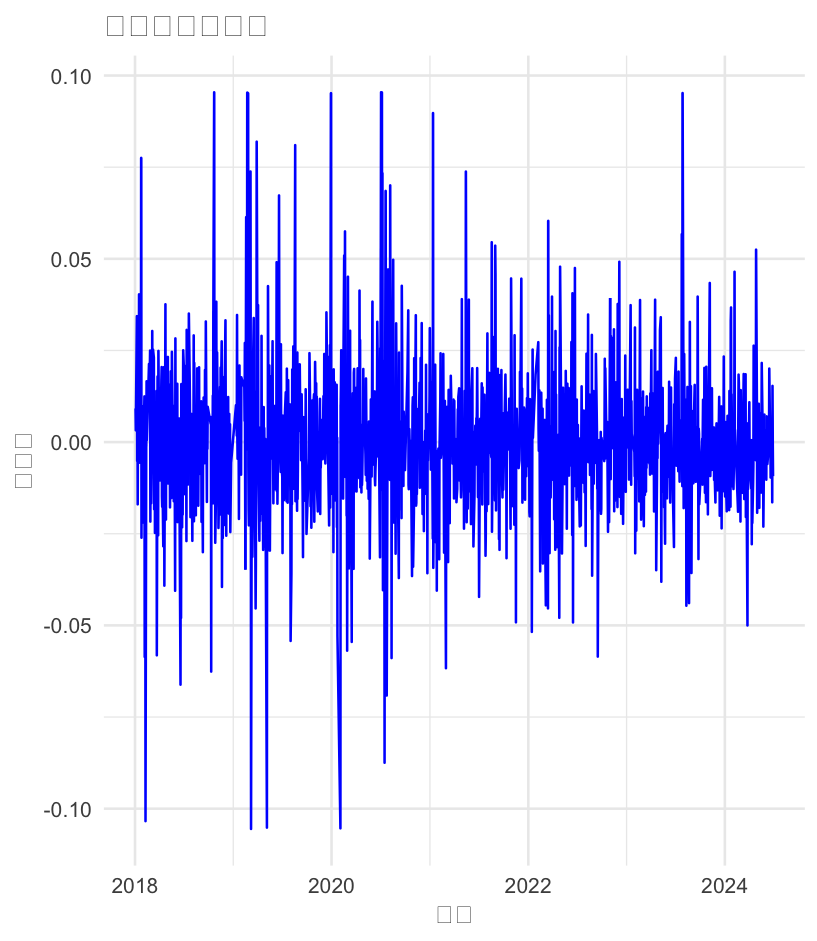
\includegraphics[width=0.5\textwidth]{A1.png}
\caption{}
\label{fig:A1}
\end{figure}

\begin{figure}[H]
\centering
\subcaptionbox{\label{}}
{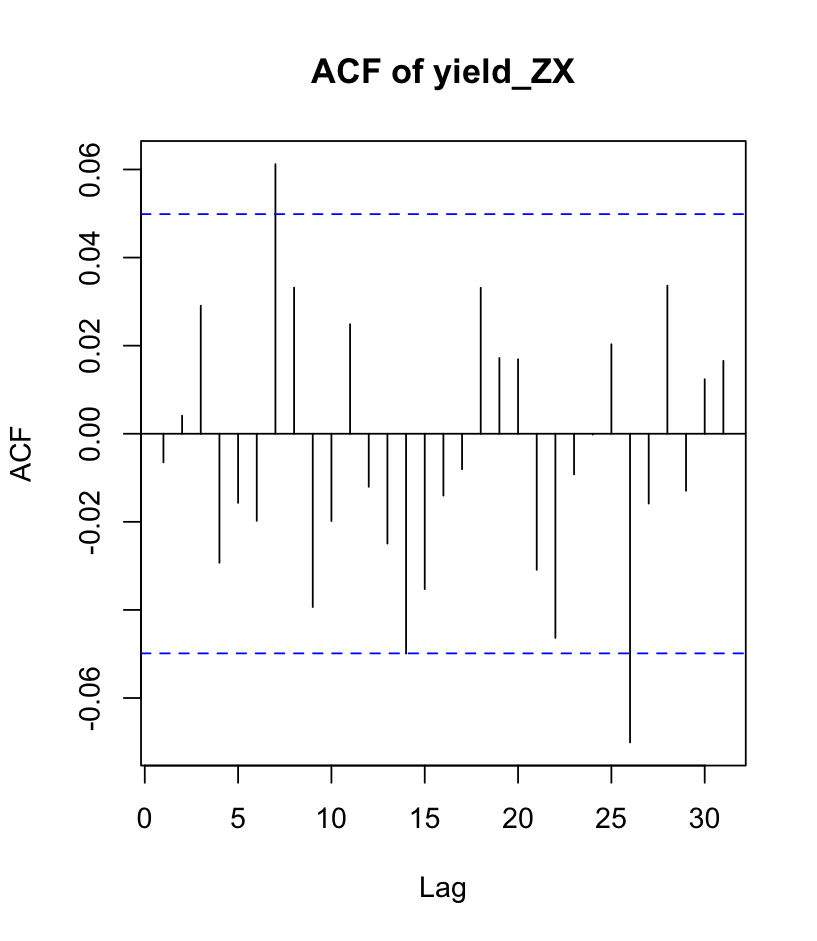
\includegraphics[width=.4\textwidth]{A2.png}}
\subcaptionbox{\label{}}
{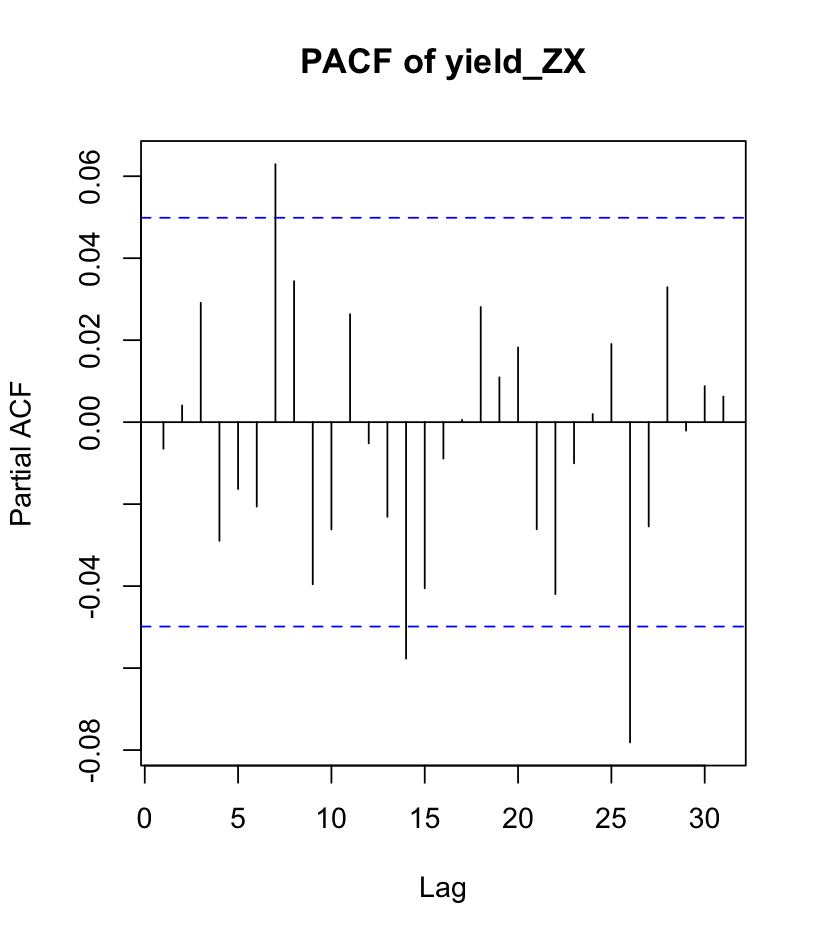
\includegraphics[width=.4\textwidth]{A3.png}}
\caption{}\label{fig:A23}
\end{figure}


除了延迟7阶、14阶、26阶之外,其他自相关、偏自相关系数均在两倍标准差范围内,说明时间序列的ACF与PACF均存在截尾性质,而拖尾性质不明显。

此外,由于之前检验出收益率时间序列中数据的变化是随机的,较难预测,我们使用auto.arima函数来自动选择出的的 ARIMA 模型为ARIMA(0,0,0) ,这是一个简单的白噪声模型,没有自回归(AR)、差分(I)或移动平均(MA)部分。针对模型ARIMA(0,0,0),求得AIC、AICc、BIC值均偏大\ref{tab:ARIMA},可知模型ARIMA(0,0,0)拟合效果不佳。

\begin{table}[H]
    \centering
    \caption{ARIMA(0,0,0)模型}
    \label{tab:ARIMA}
    \begin{tabular}{ccc}
        \toprule
        AIC & AICc & BIC \\ 
        \midrule
        -7683.64 & -7683.64 & -7678.3\\
        \bottomrule
    \end{tabular}
\end{table}

如参考论文中所述,我们使用AR(3)模型、MA(3)模型与ARMA(3,3)模型进行拟合,输出的拟合结果分别为:

\begin{itemize}
    \item AR(3)模型\ref{fig:A5}
\end{itemize}

\begin{figure}[H]
\centering
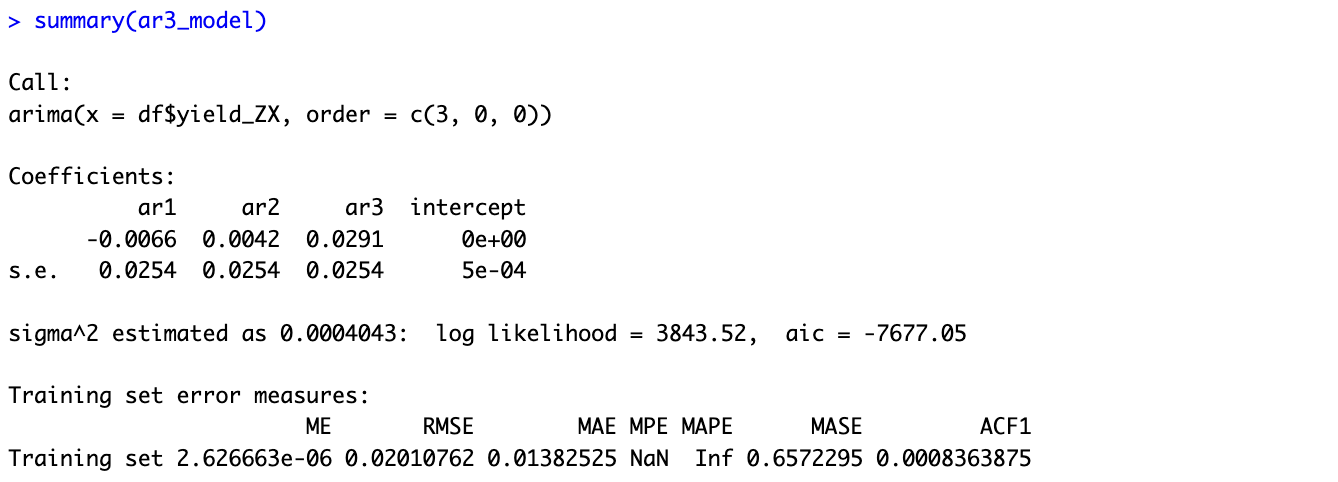
\includegraphics[width=0.75\textwidth]{A5.png}
\caption{}
\label{fig:A5}
\end{figure}

\begin{itemize}
    \item MA(3)模型\ref{fig:A6}
\end{itemize}

\begin{figure}[H]
\centering
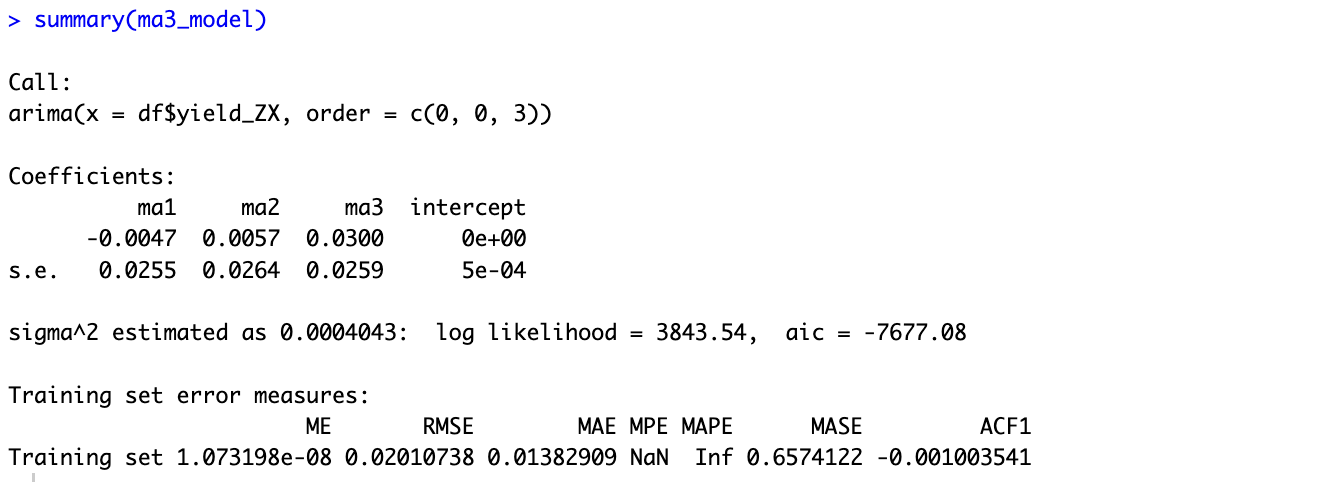
\includegraphics[width=0.75\textwidth]{A6.png}
\caption{}
\label{fig:A6}
\end{figure}

\begin{itemize}
    \item ARMA(3,3)模型\ref{fig:A7}
\end{itemize}

\begin{figure}[H]
\centering
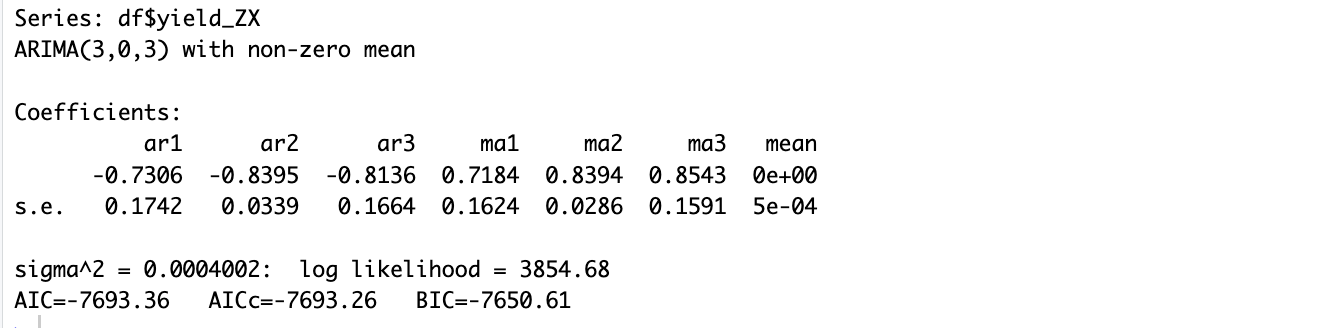
\includegraphics[width=0.75\textwidth]{A7.png}
\caption{}
\label{fig:A7}
\end{figure}

用AIC、BIC准则对ARMA(3,3)模型进行检验,结果如表\ref{tab:ARMA}所示:

\begin{table}[H]
    \centering
    \caption{ARMA(3,3)模型}
    \label{tab:ARMA}
    \begin{tabular}{ccc}
        \toprule
        AIC & AICc & BIC \\ 
        \midrule
        -7693.36 & -7693.26 & -7650.61\\
        \bottomrule
    \end{tabular}
\end{table}

相比ARIMA(0,0,0)模型,AIC、AICc值略有下降而BIC值略有上升(因为是负值),可知ARMA(3,3)模型的拟合效果与ARIMA(0,0,0)相差不多,拟合效果同样不佳。

最后,我们检验拟合残差序列是否为白噪声序列。

首先,我们获取模型拟合的残差,绘制残差分布图如下\ref{fig:AA}:

\begin{figure}[H]
\centering
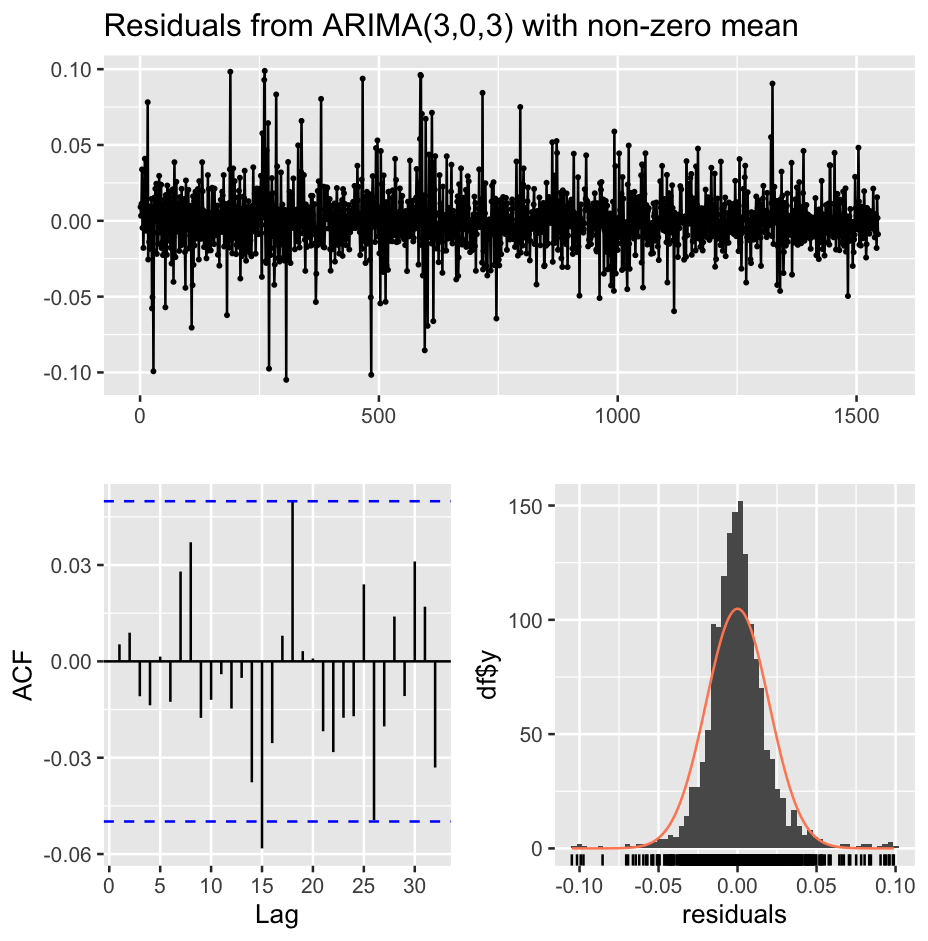
\includegraphics[width=0.65\textwidth]{AA.png}
\caption{}
\label{fig:AA}
\end{figure}

我们仍然采用Portmanteau(Q) test与Bartlett's(B)test对残差进行白噪声检验:Portmanteau(Q) test与Bartlett's(B) test 求出的$p$值分别为0.8349和0.8351,显著大于0.1。接受原假设,拒绝备择假设,说明中信证券收益率残差序列为白噪声序列,残差白噪声检验通过。

\begin{itemize}
    \item \textbf{总结:虽然残差序列为白噪声序列,但由于中信证券收益率时间序列未能如文献所述通过白噪声序列检验,采用3阶ARMA模型拟合结果较差。}
\end{itemize}

\subsection{GARCH模型}
我们使用GARCH模型对中信证券的收盘价和收益率进行分析。我们首先绘制了中信证券的收盘价和收益率的时序图。通过观察收益率的时序图,我们可以发现其具有一定的波动性,但整体上呈现出平稳的趋势。

\begin{figure}[H]
\centering
\subcaptionbox{收盘价时序图\label{}}
{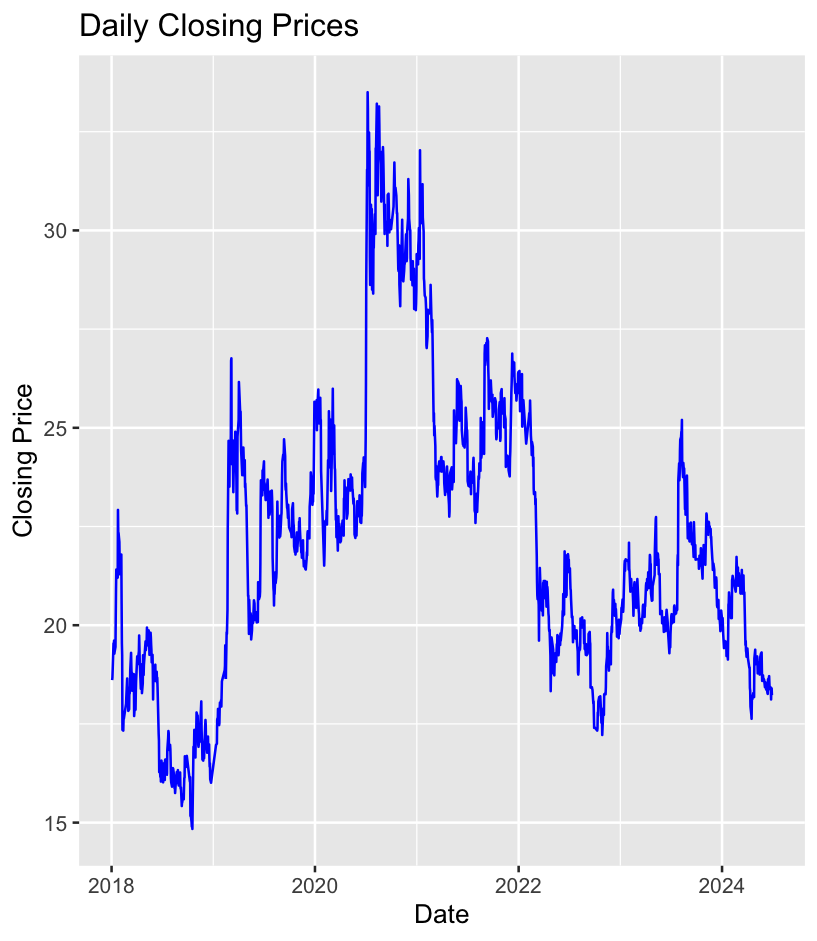
\includegraphics[width=.4\textwidth]{G1.png}}
\subcaptionbox{收益率时序图\label{}}
{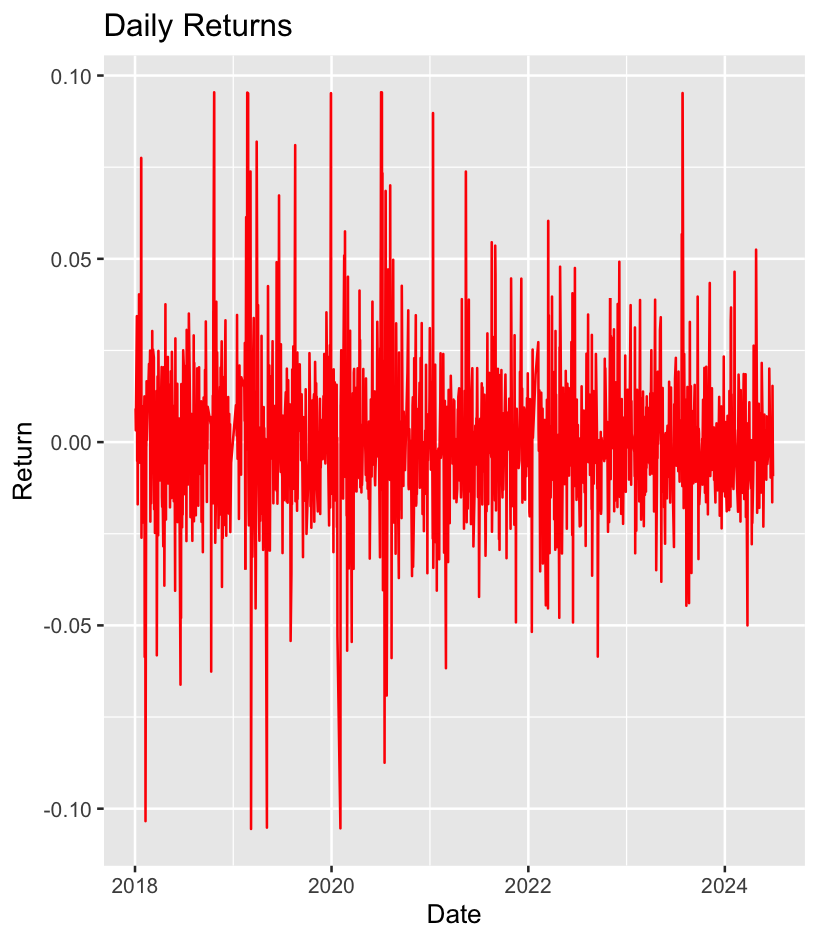
\includegraphics[width=.4\textwidth]{G2.png}}
\caption{}\label{fig:时序图}
\end{figure}

在进一步分析中,我们计算了收益率的自相关图和偏自相关图\ref{fig:ACF}。在前30阶内,收益率的自相关图中只有第7阶和第26阶超出了置信区间,这表明大多数收益率数据的自相关性并不显著。偏自相关图也呈现出类似的情况,表明收益率序列在大多数情况下是随机的。

\begin{figure}[H]
\centering
\subcaptionbox{收益率自相关图\label{}}
{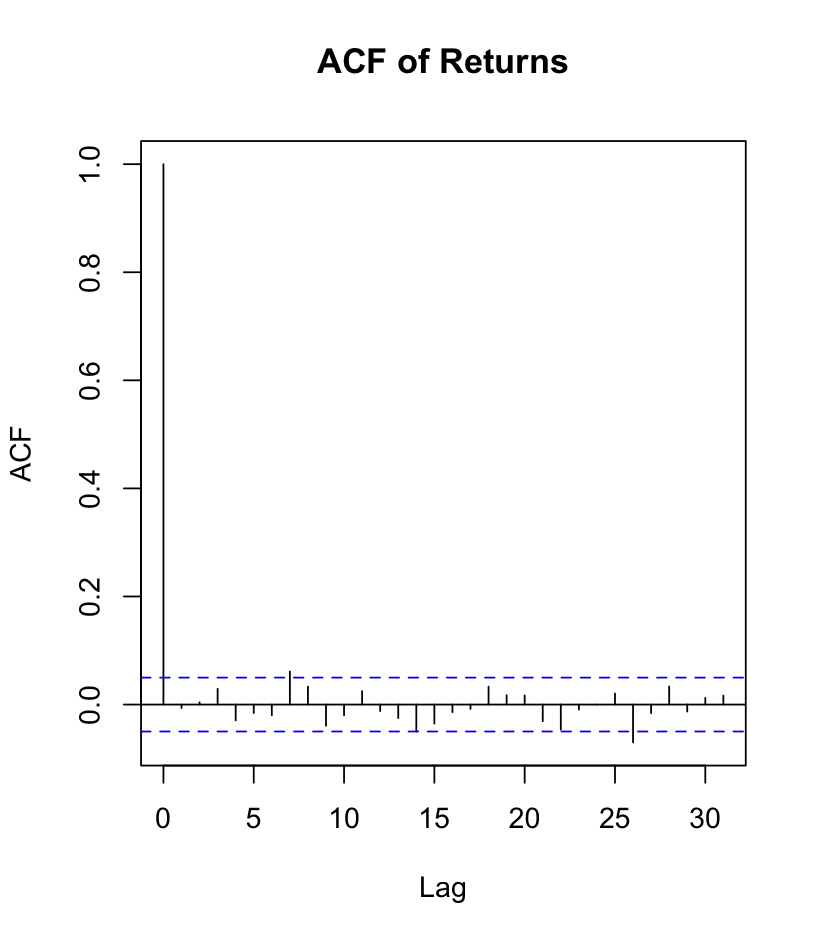
\includegraphics[width=.4\textwidth]{G3.png}}
\subcaptionbox{收益率偏自相关图\label{}}
{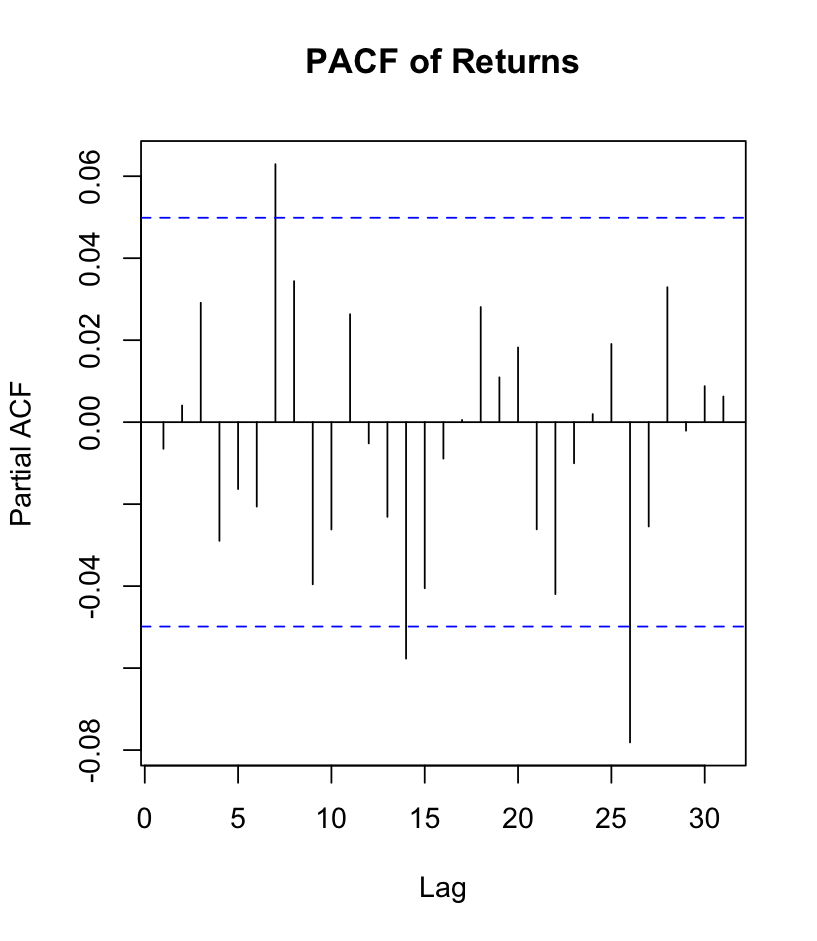
\includegraphics[width=.4\textwidth]{G4.png}}
\caption{}\label{fig:ACF}
\end{figure}

为了进一步探讨收益率的波动性特征,我们绘制了收益率平方的时序图\ref{fig:平方}、自相关图和偏自相关图\ref{fig:平方ACF}。通过观察收益率平方的时序图,我们发现其具有明显的波动性聚集特征,即波动较大的时期往往伴随着波动较小的时期。这种现象在收益率平方的自相关图和偏自相关图中也得到了体现,多个阶数的自相关系数和偏自相关系数超出了置信区间,表明收益率平方序列存在显著的自相关性。

\begin{figure}[H]
\centering
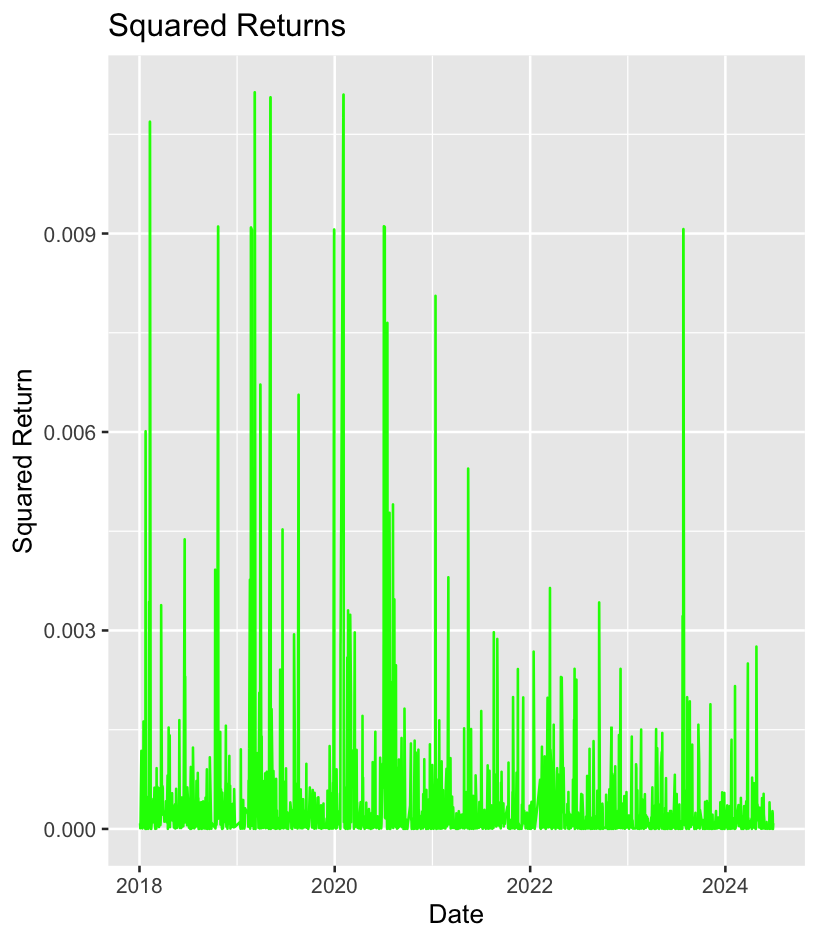
\includegraphics[width=0.5\textwidth]{G5.png}
\caption{收益率平方时序图}
\label{fig:平方}
\end{figure}

\begin{figure}[H]
\centering
\subcaptionbox{收益率平方自相关图\label{}}
{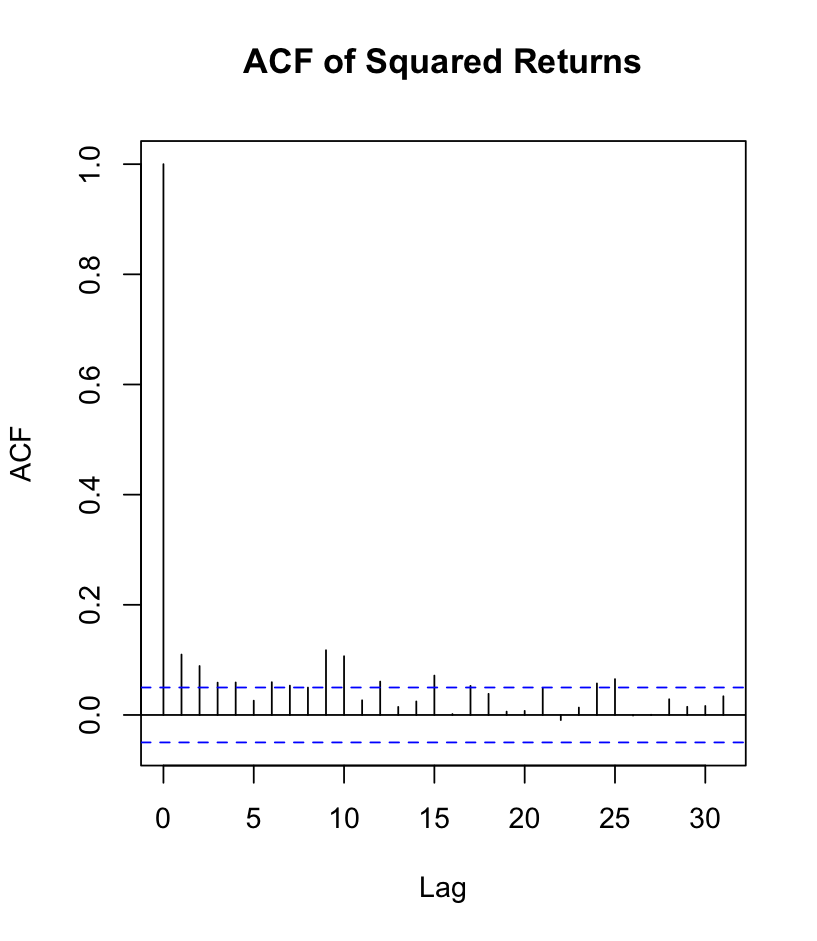
\includegraphics[width=.4\textwidth]{G6.png}}
\subcaptionbox{收益率平方偏自相关图\label{}}
{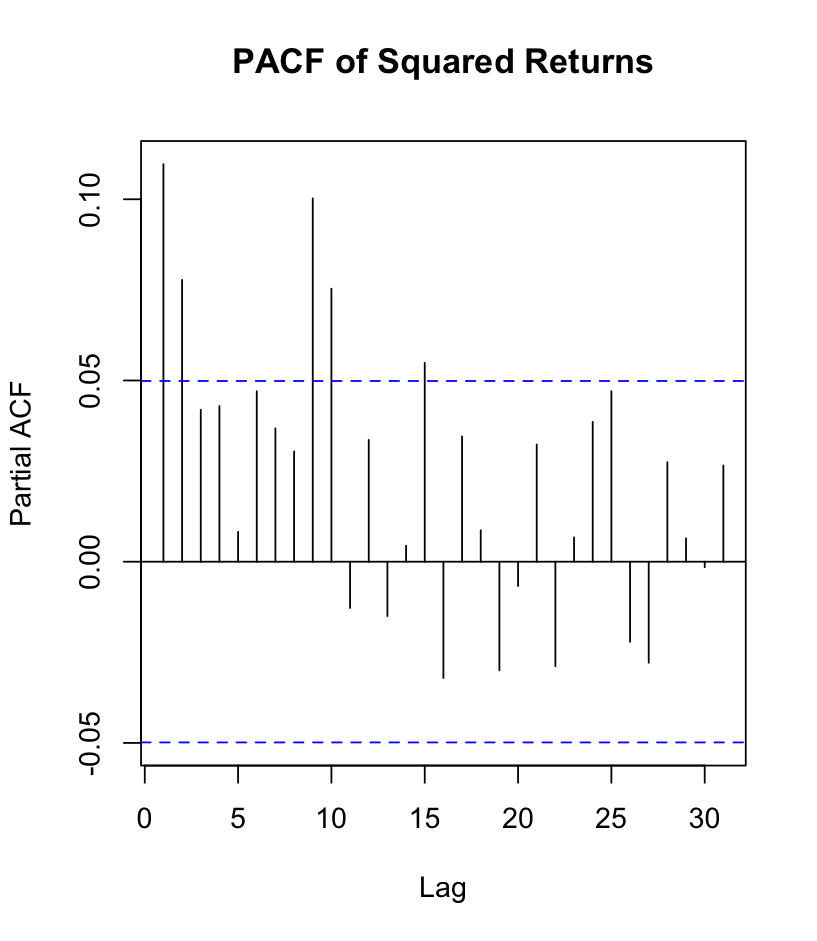
\includegraphics[width=.4\textwidth]{G7.png}}
\caption{}\label{fig:平方ACF}
\end{figure}

为了验证收益率序列中是否存在ARCH效应,我们进行了ARCH LM检验。检验结果\ref{fig:ARCHLM}显示,残差平方的自相关图和偏自相关图中也有较多的阶数超出了置信区间,进一步支持了收益率序列中存在ARCH效应的结论。

\begin{figure}[H]
\centering
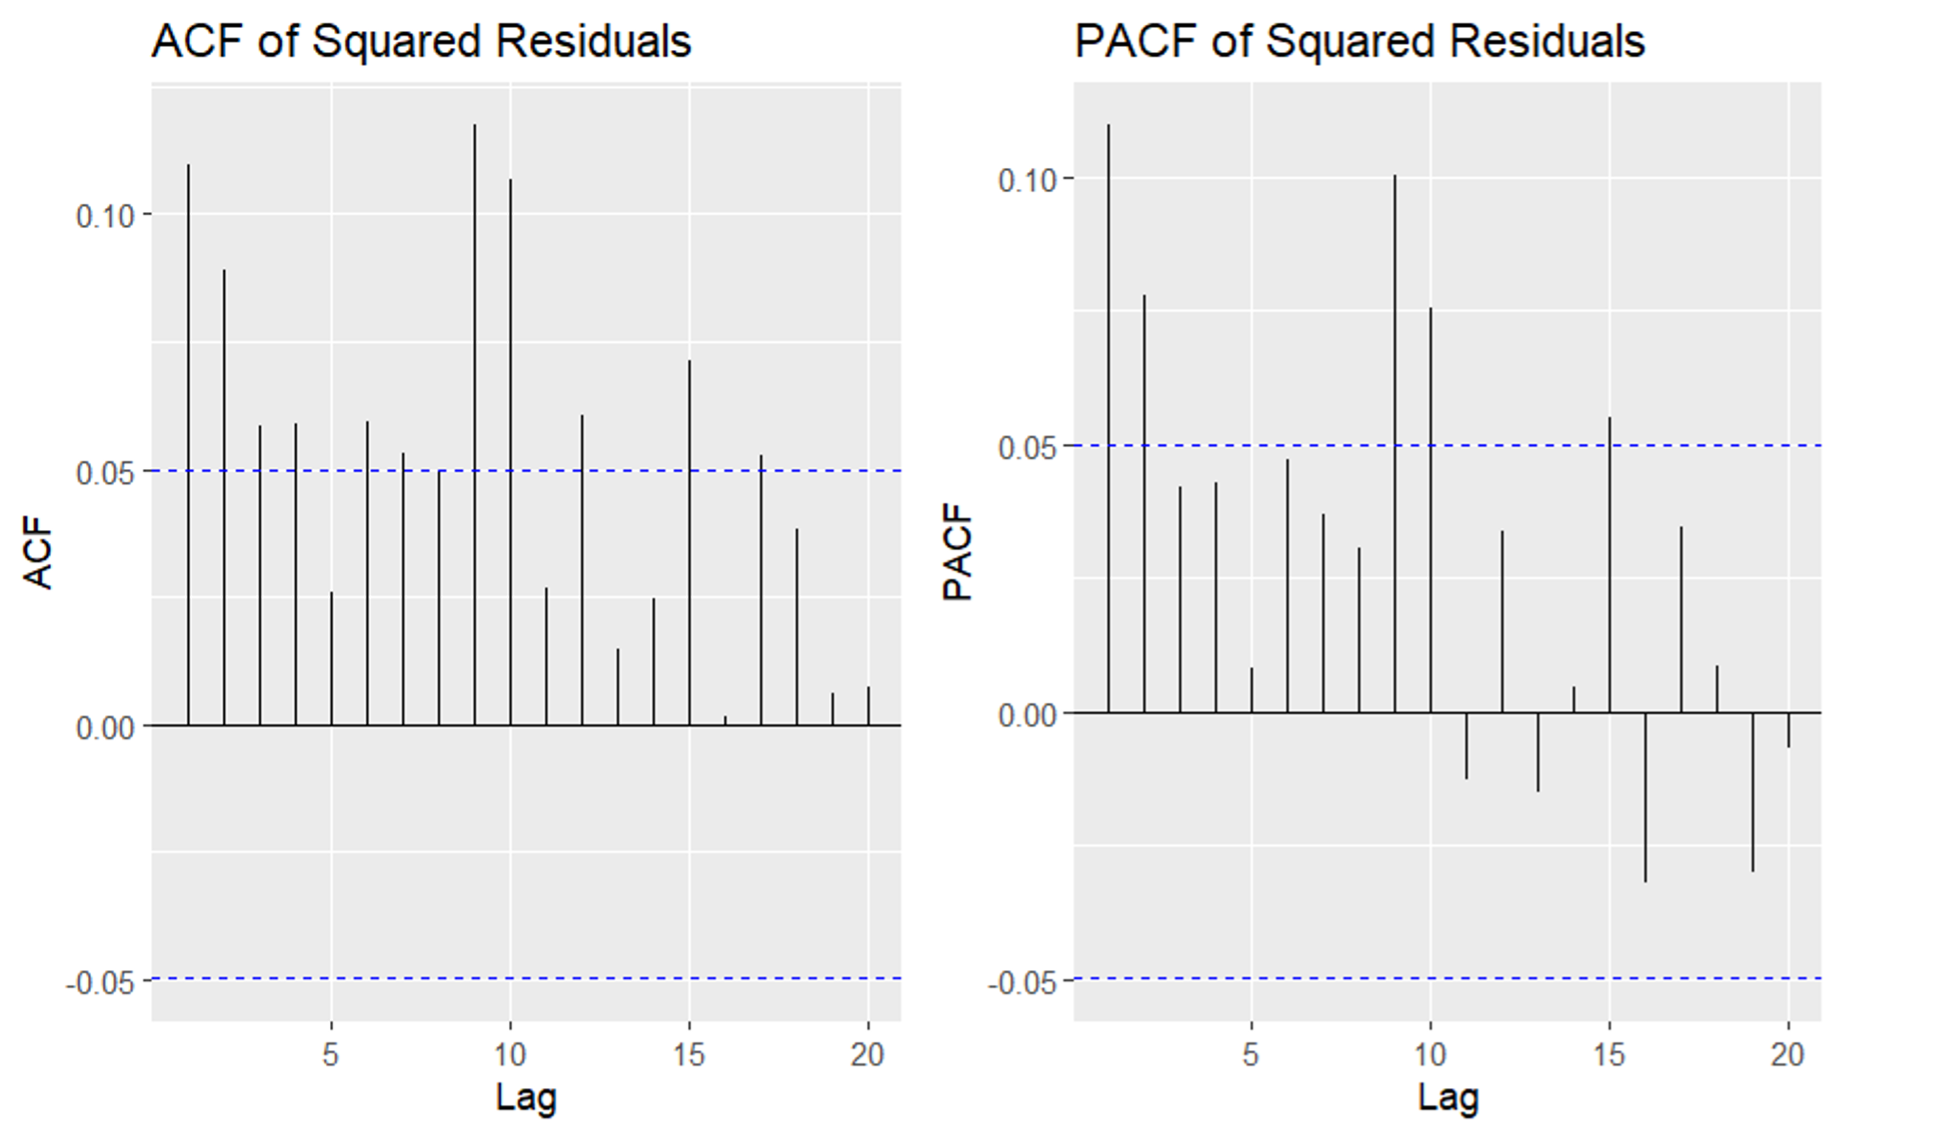
\includegraphics[width=0.9\textwidth]{GG.png}
\caption{}
\label{fig:ARCHLM}
\end{figure}

在GARCH模型的构建过程中,我们首先对中信证券收盘价的收益率进行分析。为了选择合适的模型阶数,采用了ARCH LM检验以及信息准则(AIC和BIC)进行比较。通过先前的分析,我们发现只有在$p\leq 4$的条件下,所有的$\alpha$参数才具有显著性。与此同时,模型的$q$参数必须等于0,因为任何大于0的$q$值都会导致模型中的$\alpha$和$\beta$参数不显著。因此,我们选择了$p\leq 4$作为候选模型。

为了确定最终的模型阶数,计算了不同阶数下的AIC和BIC值。结果显示,当$p=4$时,AIC和BIC的值都最小,因此最终选择了$p=4$和$q=0$作为GARCH模型的阶数。

通过表\ref{tab:AICBIC}可以看出,当滞后阶数为4时,AIC和BIC值均达到了最小值,说明在所选模型中,GARCH(4,0)模型是最优的选择。

\begin{table}[H]
    \centering
    \caption{GARCH模型的AIC和BIC值}
    \label{tab:AICBIC}
    \begin{tabular}{ccc}
        \toprule
        Lag & AIC & BIC \\ 
        \midrule
        1 & -4.9965 & -4.9861\\
        2 & -5.0108 & -4.9970\\
        3 & -5.0145 & -4.9972\\
        4 &	-5.0273 & -5.0066\\
        \bottomrule
    \end{tabular}
\end{table}

从表\ref{tab:GARCH40}中可以看出,估计值均具有较高的$t$值和较低的$p$值,表明模型参数在统计上显著。

\begin{table}[H]
    \centering
    \caption{GARCH(4,0)的拟合结果}
    \label{tab:GARCH40}
    \begin{tabular}{ccccc}
        \toprule
        参数 & 估计值 & 标准误差 & t值 & p值 \\ 
        \midrule
        $\mu$ & -0.0001 & 0.0005 & -0.1253 & 0.9003\\
        $\omega$ & 0.0003 &	0.0000 & 16.2007 & 0.0000\\
        $\alpha_{1}$ & 0.1371 & 0.0329 & 4.1642	& 0.0000\\
        $\alpha_{2}$ & 0.0611 &	0.0207 & 2.9446	& 0.0032\\
        $\alpha_{3}$ & 0.0473 &	0.0217 & 2.1823	& 0.0291\\
        $\alpha_{4}$ & 0.0959 &	0.0300 & 3.2013	& 0.0014\\
        \bottomrule
    \end{tabular}
\end{table}

对于标准化残差平方的Ljung-Box检验结果,各滞后阶数下的$p$值均大于0.05,这进一步证明模型在刻画波动性方面是有效的。

\begin{table}[H]
    \centering
    \caption{加权Ljung-Box检验结果}
    \begin{tabular}{ccc}
        \toprule
        Lag & 统计量 & $p$值\\ 
        \midrule
        Lag[1] & 0.04387 & 0.8341\\
Lag[2*(p+q)+(p+q)-1][11] & 6.3585 & 0.3889\\
Lag[4*(p+q)+(p+q)-1][19] & 13.6022 & 0.1594\\
        \bottomrule
    \end{tabular}
\end{table}

通过图\ref{fig:Nyblom}中的Nyblom稳定性检验结果可以看出,联合统计量的值为2.0197,大于5\%临界值1.68,表明整体上参数是稳定的。同时,个体统计量除了$\alpha_{3}$和$\mu$之外,其他统计量的值于10\%临界值0.35,整体参数是相对稳定的。

\begin{figure}[H]
\centering
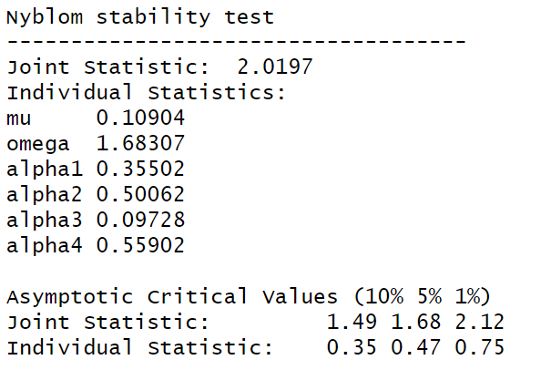
\includegraphics[width=0.7\textwidth]{Nyblom.png}
\caption{Nyblom稳定性检验}
\label{fig:Nyblom}
\end{figure}


\subsection{VAR模型}

在构建VAR模型之前,我们对三个变量进行了ADF(Augmented Dickey-Fuller)检验,结果显示$p$值小于0.01,表明三个变量均为平稳时间序列。

\begin{table}[H]
    \centering
    \caption{ADF检验}
    \label{tab:ADF}
    \begin{tabular}{ccccc}
        \toprule
        变量 & Dickey-Fuller 统计量 & 滞后阶数 & $p$值 & 备择假设 \\
        \midrule
        金融指数收益率 & -11.331 & 11 & \textless 0.01 & 平稳\\
        上证指数收益率 & -11.538 & 11 & \textless 0.01 & 平稳\\
        中信证券收益率 & -11.328 & 11 & \textless 0.01 & 平稳\\
        \bottomrule
    \end{tabular}
\end{table}

接下来,我们通过AIC(Akaike信息准则)和BIC(Bayesian信息准则)选择VAR模型的最优滞后期数,得到最优的滞后期数为1。


根据VAR模型,我们建立三个回归方程,并得到对应的估计结果:

\begin{table}[H]
    \centering
    \caption{Stock\_Return方程估计结果}
    \label{tab:VAR1}
    \begin{tabular}{ccccc}
        \toprule
        变量 & 估计值 & 标准误差 & $t$值 & $p$值 \\
        \midrule
Stock\_Return.l1    & 7.27E-02  & 5.07E-02 & 1.434  & 0.152 \\
Financial\_Index.l1 & -7.94E-02 & 7.47E-02 & -1.063 & 0.288 \\
SH\_Index.l1        & -5.24E-02 & 9.44E-02 & -0.555 & 0.579 \\
const               & -4.69E-06 & 5.12E-04 & -0.009 & 0.993 \\
        \bottomrule
    \end{tabular}
\end{table}

\begin{itemize}
    \item \textbf{回归结果解释:}
\end{itemize}

对于Stock\_Return方程,过去一期的Stock\_Return、Financial\_Index和SH\_Index对当前Stock\_Return的影响均不显著($p$值均大于0.05);方程的$R^2$较低(0.002203),说明模型对Stock\_Return的解释力较弱。


\begin{table}[H]
    \centering
    \caption{Financial\_Index方程估计结果}
    \label{tab:VAR2}
    \begin{tabular}{ccccc}
        \toprule
        变量 & 估计值 & 标准误差 & $t$值 & $p$值 \\
        \midrule
Stock\_Return.l1    & 0.1061264 & 0.042466 & 2.499  & 0.0126* \\
Financial\_Index.l1 & -0.077483 & 0.062542 & -1.239 & 0.2156  \\
SH\_Index.l1        & -0.112689 & 0.079012 & -1.426 & 0.154   \\
const               & -0.000121 & 0.000429 & -0.281 & 0.7785  \\
        \bottomrule
    \end{tabular}
\end{table}

\begin{itemize}
    \item \textbf{回归结果解释:}
\end{itemize}

对于Financial\_Index方程,过去一期的Stock\_Return对当前Financial\_Index有显著的正向影响($p$值为0.0126),表明Stock\_Return的变化对Financial\_Index有一定的预测能力;Financial\_Index和SH\_Index的滞后项对当前Financial\_Index的影响均不显著;方程的$R^2$为0.005718,略高于Stock\_Return方程,但仍较低。

\begin{table}[H]
    \centering
    \caption{SH\_Index方程估计结果}
    \label{tab:VAR3}
    \begin{tabular}{ccccc}
        \toprule
        变量 & 估计值 & 标准误差 & $t$值 & $p$值 \\
        \midrule
Stock\_Return.l1    & 7.21E-02  & 2.71E-02 & 2.657  & 0.00797** \\
Financial\_Index.l1 & -3.37E-02 & 3.99E-02 & -0.845 & 0.39852   \\
SH\_Index.l1        & -5.20E-02 & 5.05E-02 & -1.03  & 0.30332   \\
const               & -4.13E-05 & 2.74E-04 & -0.151 & 0.88007   \\
        \bottomrule
    \end{tabular}
\end{table}

\begin{itemize}
    \item \textbf{回归结果解释:}
\end{itemize}

对于SH\_Index方程,过去一期的Stock\_Return对当前SH\_Index有显著的正向影响($p$值为0.00797),表明Stock\_Return的变化对SH\_Index有一定的预测能力;Financial\_Index和SH\_Index的滞后项对当前SH\_Index的影响均不显著;方程的$R^2$为0.005186,与Financial\_Index方程相近。

\begin{itemize}
    \item \textbf{总结:VAR模型显示Stock\_Return对Financial\_Index和SH\_Index均有显著的正向影响,而Financial\_Index和SH\_Index对Stock\_Return的影响不显著。这表明Stock\_Return的变化对另外两个指数的收益率有一定的预测能力,而其他变量的滞后项对彼此的影响较小。}
\end{itemize}

\newpage
在对VAR模型残差进行自相关和偏自相关分析时,发现自相关图\ref{fig:自}中除0阶外,所有变量的所有阶数均在置信区间内,这表明残差不存在显著的自相关性。

\begin{figure}[H]
\centering
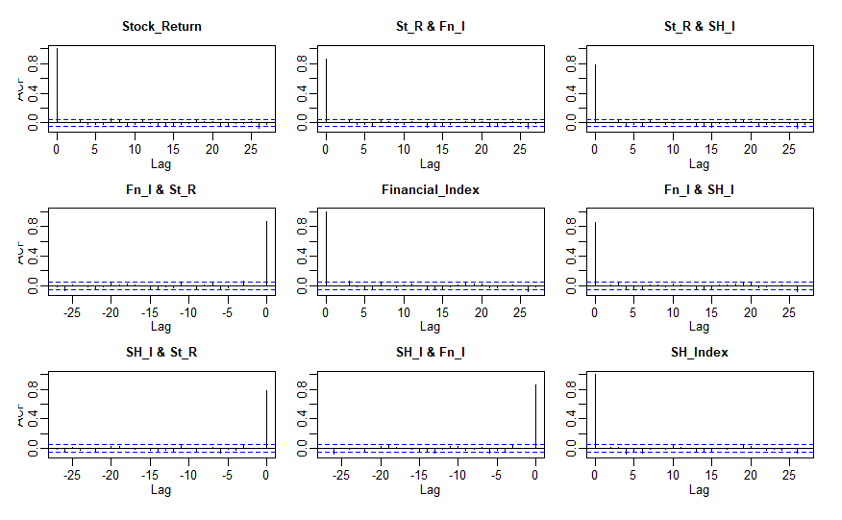
\includegraphics[width=0.9\textwidth]{VAR1.png}
\caption{自相关图}
\label{fig:自}
\end{figure}

偏自相关图\ref{fig:偏}中则表现出一些阶数在置信区间外,这表明残差存在某些滞后的偏自相关性。进一步的白噪声检验结果表明,$p$值为0.01382($\chi^2 = 111.55, df = 81$),小于0.05,拒绝白噪声假设,表明残差中存在未捕捉的依赖性。

\begin{figure}[H]
\centering
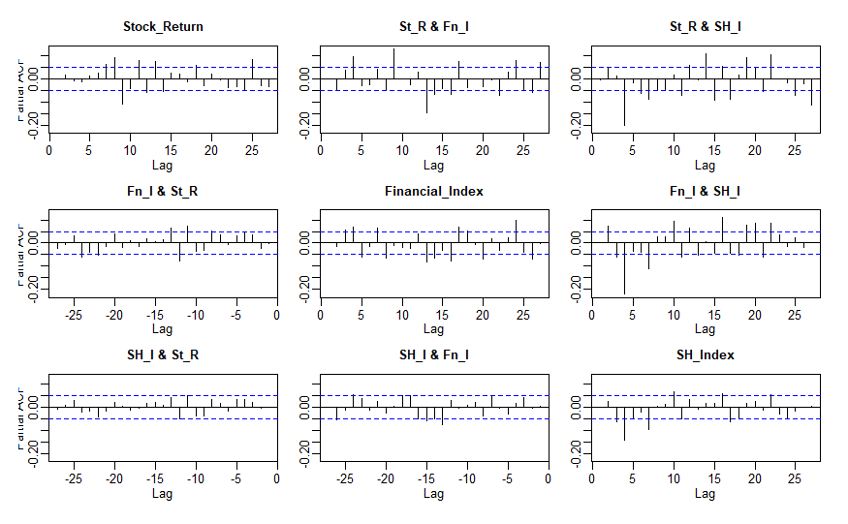
\includegraphics[width=0.9\textwidth]{VAR2.png}
\caption{偏自相关图}
\label{fig:偏}
\end{figure}


通过脉冲响应分析\ref{fig:麦},进一步考察了各变量之间的动态相互影响。结果显示,中信证券收益率(Stock\_Return)对自身、金融指数(Financial\_Index)和上证指数(SH\_Index)均产生正效应。金融指数(Financial\_Index)对中信证券收益率(Stock\_Return)产生负效应,但对自身和上证指数(SH\_Index)均产生正效应。而上证指数(SH\_Index)对中信证券收益率(Stock\_Return)和金融指数(Financial\_Index)均产生负效应,对自身则产生正效应。

\begin{figure}[H]
\centering
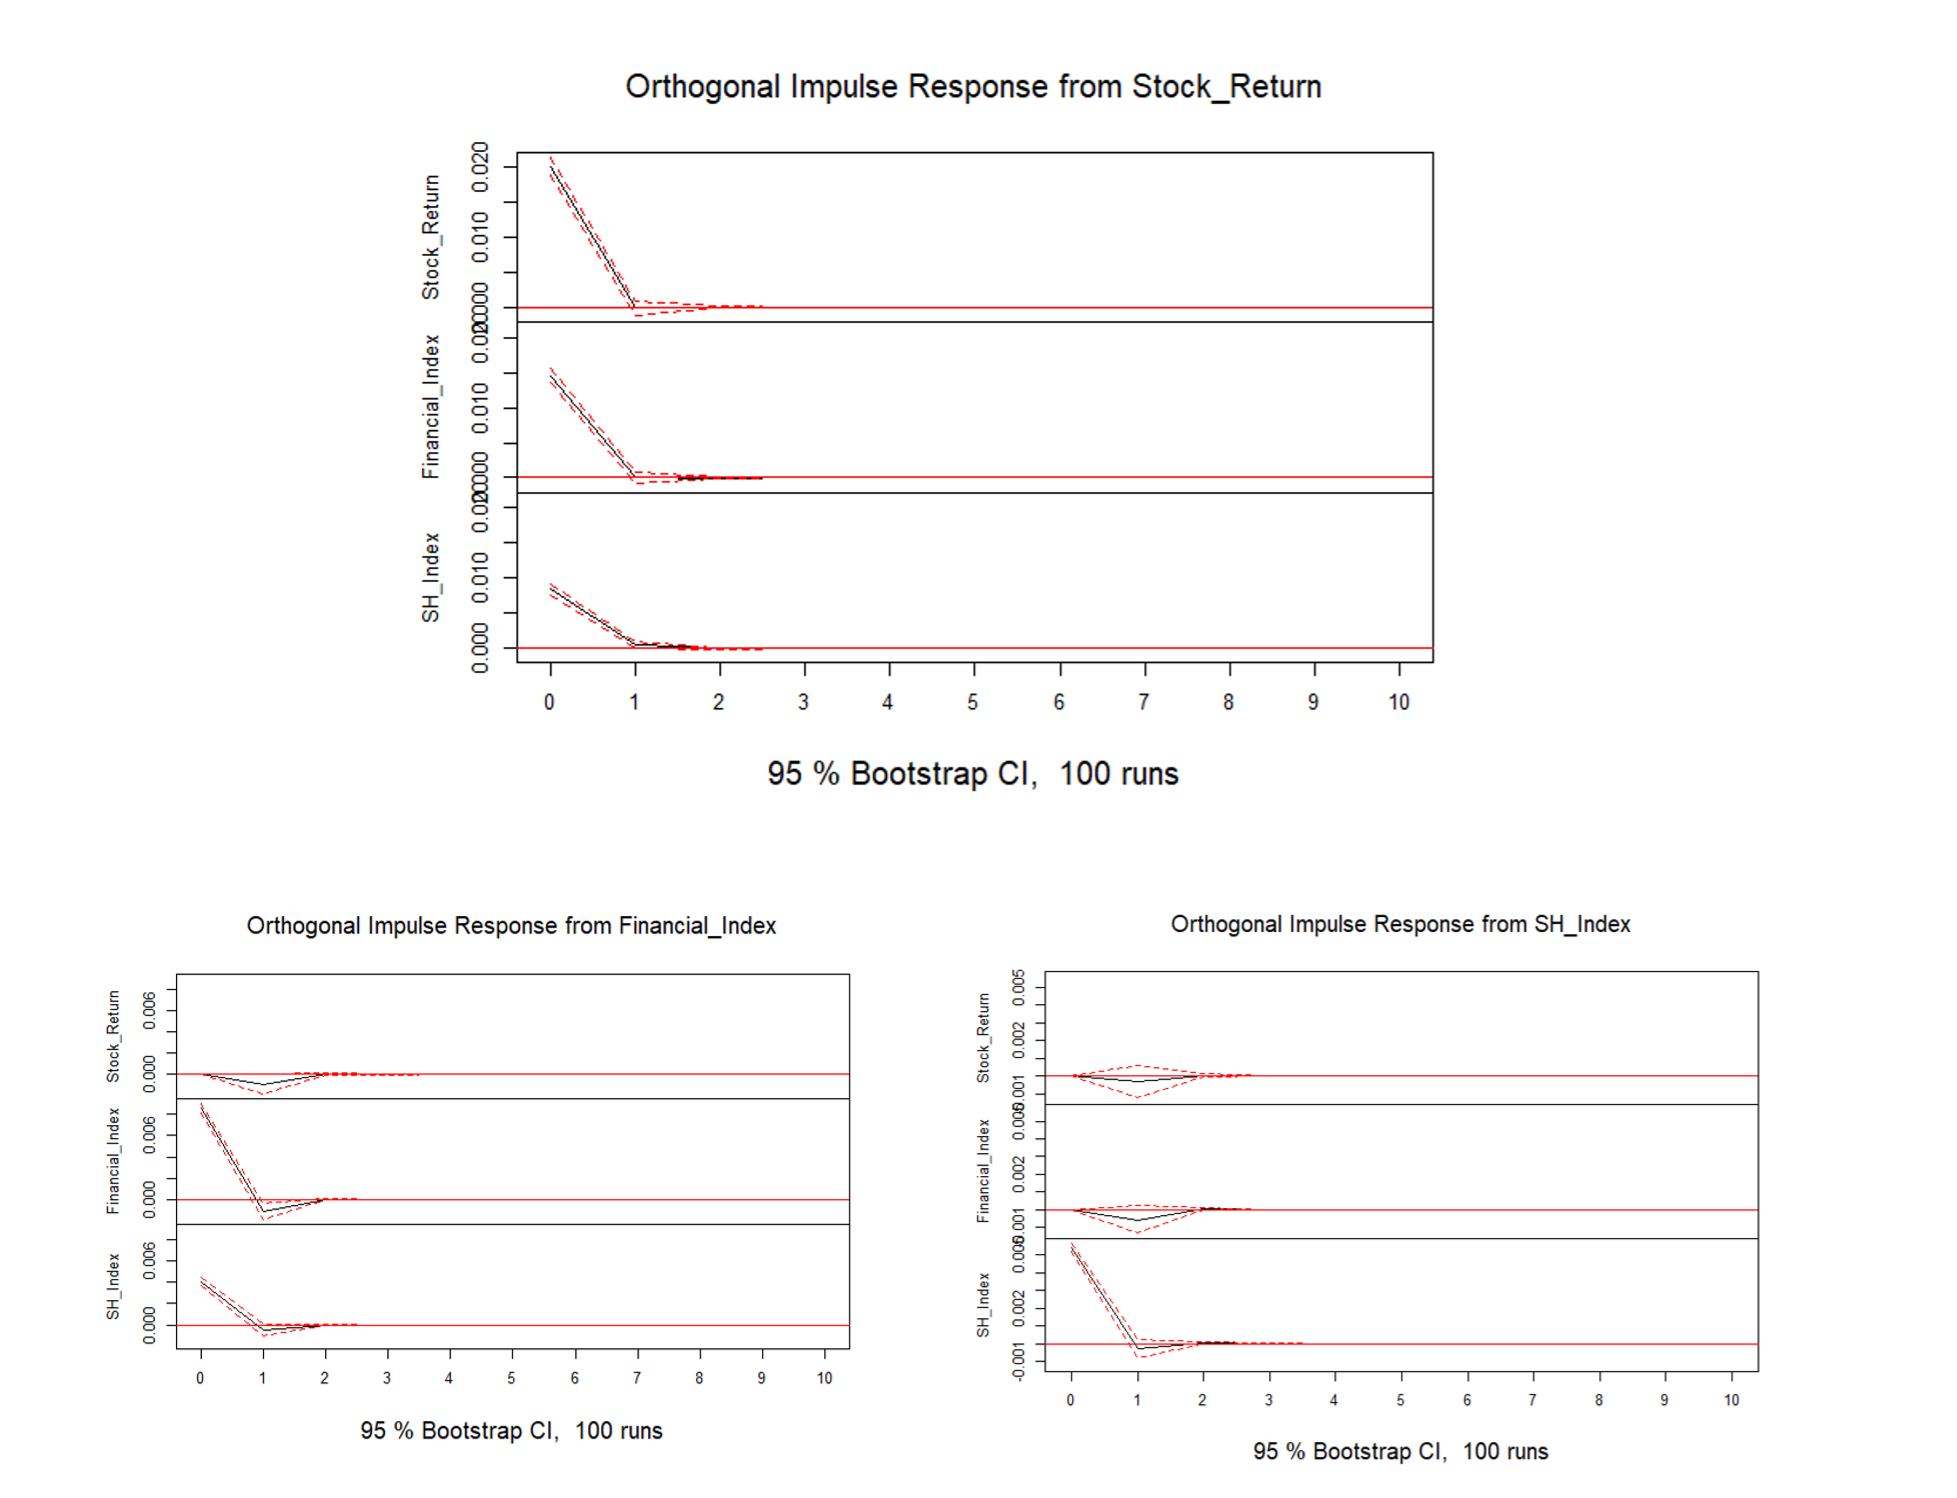
\includegraphics[width=0.9\textwidth]{VAR3.png}
\caption{脉冲响应分析}
\label{fig:麦}
\end{figure}



在这一部分,我们使用Granger因果分析来检验金融指数(Financial\_Index)和上证指数(SH\_Index)是否对中信证券收益率(Stock\_Return)具有因果关系,并进一步检验这两个变量之间是否存在即时因果关系。

首先,我们看Granger因果分析的结果,如表\ref{tab:Granger}所示。Granger因果分析的原假设是金融指数和上证指数不Granger引起中信证券收益率。结果显示$F$统计量为1.6672,自由度为2和4620,对应的$p$值为0.1889。由于$p$值大于0.05,我们无法拒绝原假设,说明在传统的显著性水平下,我们没有足够的证据表明金融指数和上证指数Granger引起中信证券收益率。

\begin{table}[H]
    \centering
    \caption{Granger因果分析}
    \label{tab:Granger}
    \begin{tabular}{ccccc}
        \toprule
       检验类型 & 统计量 & 自由度 & $p$值 & 结论\\
        \midrule
Granger因果 & $F$ = 1.6672 & $df_1$ = 2, $df_2$ = 4620 & 0.1889 & 无法拒绝原假设 \\
即时因果关系 & $\chi^2$ = 660.81 & df = 2 & \textless 2.2e-16 & 拒绝原假设 \\
        \bottomrule
    \end{tabular}
\end{table}


接下来,我们检验变量之间的即时因果关系。即时因果关系的原假设是金融指数、上证指数和中信证券收益率之间不存在即时因果关系。结果显示$\chi^2$统计量为660.81,自由度为2,对应的$p$值小于2.2e-16。由于$p$值远小于0.05,我们可以拒绝原假设,说明金融指数、上证指数和中信证券收益率之间存在显著的即时因果关系。

从Granger因果分析的结果可以看出,虽然金融指数和上证指数对中信证券收益率没有Granger因果关系,但即时因果关系检验结果却表明这三个变量之间存在显著的即时因果关系。这表明,虽然滞后的金融指数和上证指数对中信证券收益率的预测能力较弱,但在当前时点上,这三个变量之间存在强烈的联动效应。

具体来说,Granger因果分析未能发现显著的滞后效应,可能是由于变量之间的关系较为复杂,需要更多的滞后期或者其他潜在因素的影响。然而,即时因果关系检验结果却显示了这些变量在同一时点上存在显著的相互影响,可能反映了市场的瞬时反应性和高度敏感性。在金融市场中,信息传播和投资者的决策通常会迅速反映在价格变动中,导致变量之间存在显著的即时关系。

\end{document}

\begin{figure}[H]
\centering
\includegraphics[width=0.75\textwidth]{framework of macro.png}
\caption{单图}
\label{}
\end{figure}

\begin{figure}[H]
\centering
\subcaptionbox{炉温曲线示意图\label{}}
{\includegraphics[width=.4\textwidth]{framework of macro.png}}
\subcaptionbox{问题1炉温曲线\label{}}
{\includegraphics[width=.4\textwidth]{framework of macro.png}}
\caption{双图}\label{}
\end{figure}